\documentclass[12pt,thmsa]{article}

%maths
\usepackage{amsmath}   % \sideset
\usepackage{amsthm}    % for proof
\usepackage{amsfonts}  % for \mathbb
\usepackage{mathrsfs}  % for Ralph Smith's Formal Script Font
\usepackage[mathscr]{euscript} %redefine the \mathcal command to use Euler script
\usepackage{amssymb}   % \varnothing, \bigstar, \blacksquare, \clubsuit, \blacktriangleright, \diamondsuit, \spadesuit, \dagger, \checkmark

%algorithms
\usepackage{algorithm} % http://ctan.org/pkg/algorithms
\usepackage{algpseudocode}% http://ctan.org/pkg/algorithmicx

%tables
\usepackage{booktabs}  % Allows the use of \toprule, \midrule and \bottomrule in tables
\usepackage{multirow}
\usepackage{multicol}
\usepackage{tabularx}
\usepackage[table]{xcolor} % For \cellcolor
\usepackage[export]{adjustbox}

%figures
\usepackage{graphicx}  % Allows including images
\usepackage{float}     % Force figure placement in text with [H]

%tikzpicture
\usepackage{tikz}
\usepackage{scalerel}
\usepackage{pict2e}
\usepackage{tkz-euclide}
\usetikzlibrary{matrix}
\usetikzlibrary{shapes, positioning}
\usetikzlibrary{calc}
\usetikzlibrary{patterns, arrows.meta}
\usetikzlibrary{shadows}
\usetikzlibrary{external}

%pgfplots
\usepackage{pgfplots}
\pgfplotsset{compat=newest}
\usepgfplotslibrary{statistics}
\usepgfplotslibrary{fillbetween}

%colors
\usepackage{color}     % color

%other
\usepackage{cancel}
\usepackage{enumitem}
\setlist[itemize]{leftmargin=*} % global option, remove the indentation for a specific list
\usepackage{textcase}  % \MakeTextUppercase
\renewcommand{\qedsymbol}{$\blacksquare$} % change the QED symbol to a filled square
\usepackage{hyperref}

%layout
\usepackage{geometry}

\geometry{
	a4paper,
	total={170mm,257mm},
	left=20mm,
	right=20mm,
	top=20mm,
}

% Linhui added for newly defined color
\definecolor{forestgreen}{RGB}{34,139,34}

% Linhui added for Expectation and Variance
\newcommand{\Exp}{{\mathbb E}\! }
\newcommand{\Var}{\mbox{Var}\! }

% Linhui added for rename the command for empty set.
\let\oldemptyset\emptyset
\let\emptyset\varnothing

% Linhui added for empty box.
\newcommand{\emptybox}[2][0.6em]{% 
	\fbox{\rule{0pt}{#1}\hspace{#2}}%
}

% Linhui added for vertically centered boxed content
\newcommand{\vcenteredbox}[1]{%
	\begingroup
	\setbox0=\hbox{#1}%
	\parbox{\wd0}{\box0}%
	\endgroup
}

%------------------------------------------------------%
\makeatletter
\def\maketitle{%
	\par
	\hrule height 1.5pt\vspace{1ex}
	\par\noindent
	
	\begin{minipage}{0.5\textwidth}
		\scshape
		Purdue University \(\cdot\) ece 58000 \\[1ex]
		Optimization Methods \\
		Prof. Żak, Prof. Chong
	\end{minipage}
	\begin{minipage}{0.45\textwidth}
		\raggedleft
		\MakeTextUppercase{{\@title}}\\[0.3ex] % 0.2ex height space between two line
		\textit{\@author}\\[0.2ex]
		\textit{September 1, 2022}
	\end{minipage}
	\par\vspace{1ex}
	\hrule height 1.5pt\vspace{1ex}
	\par
}
\makeatother

\author{Linhui Xie}
\title{Lecture Note 02}
%------------------------------------------------------%

\begin{document}
\maketitle

\setcounter{section}{1}
\section{Convexity, Derivative\medskip}

\setcounter{section}{2}

%------------------------------------------------------%
\subsection{Lines, hyperplanes and linear varieties}

\begin{itemize}
	\item The \underline{line segment} between two points \(\boldsymbol{x}, \boldsymbol{y} \in \mathbb{R}^{n}\) is the set,
	\[
	\{{\color{forestgreen}{\boldsymbol{z}}} \in \mathbb{R}^{n}: \boldsymbol{z} = \alpha \boldsymbol{x}+(1-\alpha) \boldsymbol{y}, \alpha \in[0,1]\}.
	\]
	
	\item A hyperplane of the space \(\mathbb{R}^{n} \), is the set of all points \(\boldsymbol{x}=\left[x_{1}, x_{2}, \ldots, x_{n}\right]^{\top}\) that satisfy the linear equation
	\[
	u_{1} x_{1}+u_{2} x_{2}+\cdots+u_{n} x_{n}=v,
	\]
	where at least one of the \(u_{i}\) is nonzero. The \underline{hyperplane}  is defined by
	\[
	\left\{{\color{forestgreen}{\boldsymbol{x}}} \in \mathbb{R}^{n}: \boldsymbol{u}^{\top} \boldsymbol{x}=v\right\},
	\]where
	\[
	\boldsymbol{u}=\left[u_{1}, u_{2}, \ldots, u_{n}\right]^{\top}.
	\]
	
	\item Two \underline{half-spaces}, postive half-space and negative half-space are
	\[ H_{+}=\left\{{\color{forestgreen}{\boldsymbol{x}}} \in \mathbb{R}^{n}: \boldsymbol{u}^{\top} \boldsymbol{x} \geq v\right\}, \]
	\[ H_{-}=\left\{{\color{forestgreen}{\boldsymbol{x}}} \in \mathbb{R}^{n}: \boldsymbol{u}^{\top} \boldsymbol{x} \leq v\right\}. \]
	
	\item  A \underline{linear variety} is a set of form
	\[ \left\{\boldsymbol{x} \in \mathbb{R}^{n} : \mathbf{A}\boldsymbol{x} = \boldsymbol{b} \right\},  \]
	for some matrix \(\mathbf{A} \in \mathbb{R}^{m \times n}\) and vector \(\boldsymbol{b} \in \mathbb{R}^{n}\).
\end{itemize}

%------------------------------------------------------%
\subsection{Convex sets}

\begin{itemize}
	\item A point \(\boldsymbol{w}=\alpha \boldsymbol{u}+(1-\alpha) \boldsymbol{v}\) (where \(\alpha \in[0,1]\)) is called a \underline{convex combination} of the points \(\boldsymbol{u}\) and \(\boldsymbol{u}\).


	\item A set \(\Theta \subset \mathbb{R}^{n}\) is \underline{convex} if for all \( \boldsymbol{u}, \boldsymbol{v} \in \Theta \), the \textit{line segment} between \(\boldsymbol{u}\) and \(\boldsymbol{v}\) is in \(\Theta \). 
	
	That is, \(\Theta\) is \textit{convex} if and only if \(\alpha \boldsymbol{u}+(1-\alpha) \boldsymbol{v} \in \Theta \) for all \(\boldsymbol{u}, \boldsymbol{v} \in \Theta\) and \(\alpha \in(0,1)\). Examples of convex sets include the following:
	\begin{multicols}{2}
		\begin{itemize}
			\item The empty set
			\item A set consisting of a single point
			\item A line or a line segment
			\item A subspace
			\item A hyperplane
			\item A linear variety
			\item A half-space
			\item \(\mathbb{R}^{n}\)
		\end{itemize}
	\end{multicols}

	\item[\(\spadesuit\)] \(\mathscr{THEOREM}\)4.3 Convex subsets of \(\mathbb{R}^{n}\) have the following properties:
	
	\begin{itemize}
		\item[a.] If \(\Theta\) is a \textit{convex set} and \(\beta\) is a real number, then the set
		\[
		\beta \Theta=\{\boldsymbol{x}: \boldsymbol{x}=\beta \boldsymbol{v}, \boldsymbol{v} \in \Theta\}
		\]is also convex.
		
		\item[b.] If \(\Theta_{1}\) and \(\Theta_{2}\) are \textit{convex sets}, then the set
		\[
		\Theta_{1}+\Theta_{2}=\left\{\boldsymbol{x}: \boldsymbol{x}=\boldsymbol{v}_{1}+\boldsymbol{v}_{2}, \boldsymbol{v}_{1} \in \Theta_{1}, \boldsymbol{v}_{2} \in \Theta_{2}\right\}
		\]is also convex.
		
		\item[c.] The intersection of any collection of \textit{convex sets} is convex.
	
	\end{itemize}
	% Convexity Prove that that if \(\Theta\) and \(\Sigma\) are convex sets and \(a\) and \(b\) are real numbers, then \(a \Theta+b \Sigma\) is convex.
	
	% Convexity of intersections Prove that that if \(\Theta\) and \(\Sigma\) are convex sets and \(a\) and \(b\) are real numbers, then \( a \Theta \cap b \Sigma \) is convex.
	
	\item An \underline{extreme point} \(\boldsymbol{x}\) in a \textit{convex set} \(\Theta\), if there are no two distinct points \(\boldsymbol{u}\) and \(\boldsymbol{v}\) in \(\Theta\) such that \(\boldsymbol{x}=\alpha \boldsymbol{u}+(1-\alpha) \boldsymbol{v}\) for some \(\alpha \in(0,1)\).
	
\end{itemize}


%------------------------------------------------------%
\subsection{Differentiation rules}
\begin{itemize}
	\item A function \(f: \mathbb{R}^{n} \rightarrow \mathbb{R}\) follows,
	\[ 
	\begin{aligned}
		f(\boldsymbol{x})
		=f \left(\left[ 
		\begin{array}{c}{x_{1}} \\ {x_{2}} \\ {\vdots} \\ {x_{n}}\end{array} 
		\right] \right)
		&=a_{1} x_{1}+a_{2} x_{2}+\cdots+a_{n} x_{n}
		=\left[ 
		\begin{array}{lll}{a_{1}} & {\cdots} & {a_{n}}\end{array} 
		\right]
		\left[ 
		\begin{array}{c}{x_{1}} \\ {\vdots} \\ {x_{n}}\end{array} 
		\right] \\
		& =\left[
		\begin{array}{ccc}{} & {\boldsymbol{a}^{\top}} & {}\end{array}
		\right]
		\left[
		\begin{array}{c}{\vdots} \\ { \boldsymbol{x}} \\ {\vdots} \end{array}
		\right] 
		=\left[
		\begin{array}{ccc}{} &  {\boldsymbol{x}^{\top}} & {}\end{array}
		\right]
		\left[
		\begin{array}{c}{\vdots} \\ { \boldsymbol{a}} \\ {\vdots} \end{array}
		\right]. 
	\end{aligned}
	\]
	
	\item A matrix \(\mathbf{A} \in \mathbb{R}^{\color{black}{m} \times \color{black}{n}} \), \( \mathbf{A} \) is \(m \times n\) matrix,
	\[ \mathbf{A}
	= \left[
	\begin{array}{cccc} 
		{\vdots} & {\vdots} & & {\vdots} \\ 
		{\boldsymbol{a}_{{\color{forestgreen}*}1}} & {\boldsymbol{a}_{{\color{forestgreen}*}2}} & {\cdots} & {\boldsymbol{a}_{{\color{forestgreen}*}n}}\\ 
		{\vdots} & {\vdots} & & {\vdots}
	\end{array}
	\right] 
	= \left[
	\begin{array}{cccc}
		a_{{\color{forestgreen}1}1} & a_{{\color{forestgreen}1}2} & \cdots & a_{{\color{forestgreen}1}n} \\
		a_{{\color{forestgreen}2}1} & a_{{\color{forestgreen}2}2} & \cdots & a_{{\color{forestgreen}2}n} \\
		\vdots & \vdots & \ddots & \vdots \\
		a_{{\color{forestgreen}m}1} & a_{{\color{forestgreen}{\color{forestgreen}1}}2} & \cdots & a_{{\color{forestgreen}m}n} \\
	\end{array}
	\right]
	=\left[
	\begin{array}{c}{\boldsymbol{a}_{{\color{forestgreen}1}}^{\top}} \\
		\boldsymbol{a}_{{\color{forestgreen}2}}^{\top} \\
		{\vdots} \\ 
		{\boldsymbol{a}_{{\color{forestgreen}m}}^{\top}}
	\end{array}
	\right].
	\]
	
	\item A function \(\boldsymbol{g}: \mathbb{R}^{n} \rightarrow \mathbb{R}^{m}\) and a matrix \(\mathbf{A} \in \mathbb{R}^{\color{black}{m} \times \color{black}{n}} \), \( \mathbf{A} \boldsymbol{x} \) is a column vector whose element is a scalar \(g_{\star}(\boldsymbol{x})\). 
	\[ \mathbf{A} \boldsymbol{x}
	=\left[
	\begin{array}{c}{\boldsymbol{a}_{1}^{\top}} \\ {\vdots} \\ {\boldsymbol{a}_{m}^{\top}}\end{array}
	\right] \boldsymbol{x}
	=\left[
	\begin{array}{c}{
			\boldsymbol{a}_{1}^{\top} \boldsymbol{x}} \\ 
		{\vdots} \\ 
		{\boldsymbol{a}_{m}^{\top}\boldsymbol{x}}
	\end{array}
	\right]
	=\left[
	\begin{array}{c}{
		\boxed{ a_{11} x_{1}+a_{12} x_{2}+\cdots+a_{1 n} x_{n}} } \\ 
		{\vdots} \\ 
		\boxed{ {a_{m 1} x_{1}+a_{m 2} x_{2}+\cdots+a_{m n} x_{n}} }
	\end{array}
	\right]
	=\left[
	\begin{array}{c}{
			g_{1}(\boldsymbol{x})} \\ 
		{\vdots} \\ 
		{g_{m}(\boldsymbol{x})}
	\end{array}
	\right]
	= \boldsymbol{g}(\boldsymbol{x}).
	\]

	\item To be noted, in this course, we write the \textbf{derivative} \(D f(\boldsymbol{x}) \) as a {\color{red}{row vector}}, and write the \textbf{gradient} \( \nabla f(\boldsymbol{x}) \) as a {\color{blue}{column vector}}.
		
\end{itemize}

\newpage

\begin{center}
	Types of Matrix Derivatives\footnote{Ref: Thomas P. Minka, \href{https://tminka.github.io/papers/matrix/minka-matrix.pdf}{``Old and New Matrix Algebra Useful for Statistics''}, 2000}
\end{center}
\[
\noindent\hspace*{-1.2cm}% Move table to the left
\begin{aligned}
	\begin{array}{|c|cl|cc|cc|}
		\hline
		\multirow{2}{*}{ \text { Types }} 
			& \multicolumn{2}{c|}{\text{Scalar}} 
			& \multicolumn{2}{c|}{\text{Vector}} 
			& \multicolumn{2}{c|}{\text{Matrix}} \\  % Row 1
		\cline{2-7} 
		{}	
			&  \multicolumn{2}{c|}{ \vcenteredbox{\fbox{\vspace{1em}\hspace{1em}}} } 
			& \multicolumn{2}{c|}{ \vcenteredbox{\fbox{\vspace{1em}\hspace{1em}}} } 
			& \multicolumn{2}{c|}{ \vcenteredbox{\fbox{\vspace{1em}\hspace{1em}}} } \\ % Row 2
		\hline
		\fbox{\vspace{1em}\hspace{1em}}
			& \multirow{2}{*}{ \( \frac{\mathrm{d} y}{\mathrm{d} x} \) }  
			& \cellcolor{gray!20}
			& \multirow{2}{*}{ 
					\( \frac{\mathrm{d} \boldsymbol{y}}{\mathrm{d} x}=\left[\frac{\partial y_i}{\partial x}\right] \) 
				}
			& \cellcolor{gray!20} 
			& \multirow{2}{*}{ 
				\(\frac{\mathrm{d} \mathbf{Y}}{\mathrm{d} x}=\left[\frac{\partial y_{i j}}{\partial x}\right]\)} 
			& \cellcolor{gray!20} \\  % Row 3
		\cline{1-1} 
		\text{Scalar} 
			& 
			& \hspace{1.2cm} \multirow{-2}{*}{ \cellcolor{gray!20}
				\( \frac{\mathrm{d} f(x)}{\mathrm{d} x} \)}  \hspace{1.5cm} (1)
			& 
			& \hspace{0.9cm} \cellcolor{gray!20} \multirow{-2}{*}{ 
				\( \frac{\mathrm{d}  \boldsymbol{g}(t)}{\mathrm{d} t} \) 
			}  \hspace{0.6cm} (3) 
			&  
			& \cellcolor{gray!20} \multirow{-2}{*}{ 
				\(\frac{\mathrm{d}  \mathbf{A}(t)}{\mathrm{d} t}\) 
			} \\  % Row 4
		\hline 
		{}
			& 
			& \cellcolor{gray!20}
 			&
 			& \cellcolor{gray!20} 
 			& 
 			& \\  % Row 5
		\fbox{\vspace{1em}\hspace{1em}} 
			& \multirow{2}{*}{ \(\frac{\mathrm{d} y}{\mathrm{d} \boldsymbol{x}}=\left[\frac{\partial y}{\partial x_j}\right]\) }
			& \cellcolor{gray!20}\multirow{-2}{*}{ 
				\(D_{\boldsymbol{x}} f(\boldsymbol{x}) =\left[ \cdot \cdot \frac{\partial f(\boldsymbol{x})}{\partial x_j} \cdot \cdot \right] \)}
			& \multirow{2}{*}{ \( \frac{\mathrm{d} \boldsymbol{y}}{\mathrm{d} \boldsymbol{x}}=\left[\frac{\partial y_i}{\partial x_j}\right]\) }
			&  \cellcolor{gray!20} 
			& 
			& \\  % Row 6
		\cline{1-1}
		\text{Vector} 
			& 
			& \cellcolor{gray!20} 
			& 
			& \cellcolor{gray!20}\multirow{-2}{*}{ \( D_{\boldsymbol{x}} \boldsymbol{g}(\boldsymbol{x}) =\left[\frac{\partial g_i(\boldsymbol{x})}{\partial x_j}\right] \)} 
			& 
			&  \\  % Row 7
		{}
			&
			& \cellcolor{gray!20} \hspace{3.8cm} (2)
			& 
			& \cellcolor{gray!20} \hspace{2.6cm} (4) 
			& 
			& \\  % Row 8
		{}
			& 
			&\cellcolor{gray!20} \multirow{-3}{*}{ \(\nabla_{\boldsymbol{x}} f(\boldsymbol{x}) =\left[\begin{array}{c} 
					\cdot \\ \frac{\partial f(\boldsymbol{x})}{\partial x_j} \\ \cdot  \end{array}
				\right]\) }
			&
			& \cellcolor{gray!20}  
			& 
			& \\ [0.1cm] % adding extra space after the row  % Row 9
		\hline
		\fbox{\vspace{1em}\hspace{1em}}
			& \multirow{2}{*}{ \( \frac{\mathrm{d} y}{\mathrm{d} \mathbf{X}}=\left[\frac{\partial y}{\partial x_{j i}}\right] \) }
			& \cellcolor{gray!20} 
			& 
			& 
			& 
			& \\  % Row 10
		\cline{1-1} \text{Matrix} 
			& 
			& \hspace{0.6cm} \cellcolor{gray!20}\multirow{-2}{*}{ \( D_{\mathbf{X}} f=\left[\frac{\partial f}{\partial x_{j i}}\right] \) } 
			& 
			& 
			& 
			&\\  % Row 11
		\hline
	\end{array}
\end{aligned}
\]

\begin{itemize}
	\item[({\bf{1}})] Given \(f: \mathbb{R} \rightarrow \mathbb{R}\), if the limit exists, the derivative of \(f\) is a function \(f^{\prime}: \mathbb{R} \rightarrow \mathbb{R}\) given by
	\[
	D_{x}(f(x)) = \frac{\mathrm{d} f}{\mathrm{d} x} = f^{\prime}(x)=\lim _{h \rightarrow 0} \frac{f(x+h)-f(x)}{h}.
	\]
	
	\item[({\bf{2}})] Given \(f: \mathbb{R}^{n} \rightarrow \mathbb{R}\), consider a scalar \( f(\boldsymbol{x}) = a_{1} x_{1}+a_{2} x_{2}+\cdots+a_{n} x_{n} =  \boldsymbol{a}^{\top} \boldsymbol{x}\).

	For \textbf{derivative} rule (2), 
	\[ 
	{\color{red}{D_{\boldsymbol{x}}}} { f(\boldsymbol{x}) } =
	{\color{black}{D(}}{ \boldsymbol{a}^{\top} \boldsymbol{x} }{\color{black})} 
	= 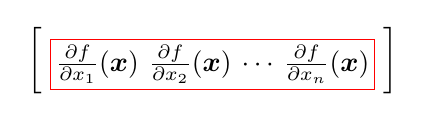
\begin{tikzpicture}[baseline=(current bounding box.center)]
			\matrix (m) [matrix of math nodes, inner sep=1.8pt, row sep=0pt, left delimiter={[},right delimiter={]}] {
				\frac{\partial f}{\partial x_1} (\boldsymbol{x}) & \frac{\partial f}{\partial x_2}(\boldsymbol{x}) & \cdots & \frac{\partial f}{\partial x_n}(\boldsymbol{x}) \\
			};
			\draw[red] (m-1-1.north west) rectangle (m-1-4.south east);
		\end{tikzpicture}
	=\left[\begin{array}{cccc}
		a_{1} & a_{2} &  \cdots & a_{n}
	\end{array}
	\right] = {\color{red}{ \boldsymbol{a}^{\top} }}.
	\]

	For \textbf{gradient} rule (2), \underline{if \(f: \mathbb{R}^{n} \rightarrow \mathbb{R}\) is differentiable}, then the \textit{gradient} of \(f\) is a function \(\nabla f: \mathbb{R}^{n} \rightarrow \mathbb{R}^{n}\) given by
	\[  {\color{blue}{\nabla}_{\boldsymbol{x}} } f(\boldsymbol{x})
	= 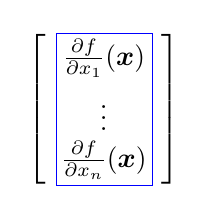
\begin{tikzpicture}[baseline=(current bounding box.center)]
			\matrix (m) [matrix of math nodes, inner sep=2pt, left delimiter={[},right delimiter={]}, nodes in empty cells] {
				\frac{\partial f}{\partial x_1} (\boldsymbol{x}) \\
				|[minimum height=0.5cm]|  \vdots \\
				\frac{\partial f}{\partial x_n} (\boldsymbol{x}) \\
			};
			\draw[blue] (m-1-1.north west) rectangle (m-3-1.south east);
		\end{tikzpicture}
	= \left[ \begin{array}{c} a_1  \\ \vdots \\ a_n \end{array} \right]
	= {\color{blue}{ \boldsymbol{a} }}
	= D_{\boldsymbol{x}} f(\boldsymbol{x}) ^{\top}.
	\] 

	\item[({\bf{3}})] Given \(\boldsymbol{g}: \mathbb{R} \rightarrow \mathbb{R}^m \), here \(t \in \mathbb{R} \) is a scalar. \(\boldsymbol{g}(t)\) is a column vector.
	\[
	\begin{aligned}
		\boldsymbol{g}(t) =
		\left[
		\begin{array}{c}
			g_{1}(t) \\
			\vdots \\
			g_{m}(t)
		\end{array}
		\right], \quad
		D_{t} \boldsymbol{g}(t) & =\left[
		\begin{aligned}
			\frac{\mathrm{d}}{\mathrm{d} t}g_{1}(t) \\
			\vdots \qquad \\
			\frac{\mathrm{d}}{\mathrm{d} t}g_{m}(t)
		\end{aligned}
		\right] =\left[\begin{array}{c}
			g_{1}^{\prime}(t) \\
			\vdots \\
			g_{m}^{\prime}(t)
		\end{array}\right].  \\
	\end{aligned}
	\]

	\item[({\bf{4}})] Consider \(\boldsymbol{g}: \mathbb{R}^{n} \rightarrow \mathbb{R}^m \),  here \( \boldsymbol{x} \in  \mathbb{R}^n \) is a vector. Since \(g_{i}(\boldsymbol{x})\) is a scalar, \(\boldsymbol{g}=\left[g_1, \ldots, g_m\right]^{\top} \), \(\boldsymbol{g}(\boldsymbol{x})\) is a column vector.
	\[
	\begin{aligned}
		\boldsymbol{g} \left( \boldsymbol{x} \right)=
		\left[
		\begin{array}{c}
			g_{1}( \boldsymbol{x} ) \\
			g_{2}( \boldsymbol{x} ) \\
			\vdots \\
			g_{m}( \boldsymbol{x} )
		\end{array}
		\right], 
		D_{\boldsymbol{x}} \boldsymbol{g}\left( \boldsymbol{x} \right) & =\left[
		\begin{array}{c}
			 { \color{red}D_{\boldsymbol{x}} } g_{1}\left( x_1,x_2,\cdots,x_n \right) \vspace{0.3cm} \\
			 { \color{red}D_{\boldsymbol{x}} } g_{2}\left( x_1,x_2,\cdots,x_n \right)  \\
			\vdots \\
			 { \color{red}D_{\boldsymbol{x}} } g_{m}\left( x_1,x_2,\cdots,x_n \right) 
		\end{array}
		\right]
		= 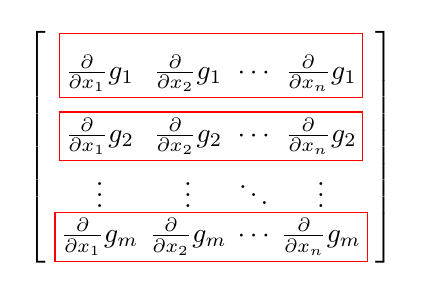
\begin{tikzpicture}[baseline=(current bounding box.center)]
			\matrix [matrix of math nodes, inner sep=2pt, left delimiter={[},right delimiter={]}] (m) {
				|[minimum height=1cm]| \frac{\partial}{\partial x_1} g_1 & \frac{\partial}{\partial x_2} g_1 & \cdots & \frac{\partial}{\partial x_n} g_1 \\
				\frac{\partial}{\partial x_1} g_2 & \frac{\partial}{\partial x_2} g_2 & \cdots & \frac{\partial}{\partial x_n} g_2 \\
				\vdots & \vdots & \ddots & \vdots \\
				\frac{\partial}{\partial x_1} g_m & \frac{\partial}{\partial x_2} g_m & \cdots & \frac{\partial}{\partial x_n} g_m \\
			};
			\draw[red] (m-1-1.north west) rectangle (m-1-4.south east);
			\draw[red] (m-2-1.north west) rectangle (m-2-4.south east);
			\draw[red] (m-4-1.north west) rectangle (m-4-4.south east);
		\end{tikzpicture}
		= \mathbf{J}.
	\end{aligned}
	\]
	The matrix \(\mathbf{J}\) is called the \underline{Jacobian matrix}, or derivative matrix, of function \(\boldsymbol{g}\).
\end{itemize}

\newpage
	
\begin{itemize}
	\item If all elements in \(\boldsymbol{g}( \boldsymbol{x} )\) are linear combination of \(\boldsymbol{x}\),
	\[ \boldsymbol{g}( \boldsymbol{x} )
	=\left[
	\begin{array}{c}{
			g_{1}(\boldsymbol{x})} \\ 
		{\vdots} \\ 
		{g_{m}(\boldsymbol{x})}
	\end{array}
	\right]
	=\left[
	\begin{array}{c}{
			a_{11} x_{1}+a_{12} x_{2}+\cdots+a_{1 n} x_{n}} \\ 
		{\vdots} \\ 
		{a_{m 1} x_{1}+a_{m 2} x_{2}+\cdots+a_{m n} x_{n}}
	\end{array}
	\right]
	=\left[
	\begin{array}{c}{
			\boldsymbol{a}_{1}^{\top} \boldsymbol{x}} \\ 
		{\vdots} \\ 
		{\boldsymbol{a}_{m}^{\top}\boldsymbol{x}}
	\end{array}
	\right]
	=\left[
	\begin{array}{c}{\boldsymbol{a}_{1}^{\top}} \\ {\vdots} \\ {\boldsymbol{a}_{m}^{\top}}\end{array}
	\right] \boldsymbol{x}
	= \mathbf{A} \boldsymbol{x}.
	\]
	
	Then, the derivative of \(\mathbf{A} \boldsymbol{x}\) is equivalent to \( D_{\boldsymbol{x}} \boldsymbol{g}( \boldsymbol{x} ) \),
	\[ {\color{red}D( } \boldsymbol{g}( \boldsymbol{x} ) {\color{red}{ ) }} 
	= \underbrace{\frac{\mathrm{d}}{\mathrm{d} \boldsymbol{x}} \left(  \mathbf{A} \boldsymbol{x} \right)}_{\text{\begin{tabular}{c} Notation not used \\ in this course \end{tabular}}}
	= {\color{black}{ D( }} \mathbf{A} \boldsymbol{x} {\color{black}{ ) }} 
	= \left[
		\begin{array}{c}
			{\color{black}{D(}}{ \boldsymbol{a}_{1}^{\top} \boldsymbol{x} }{\color{black})} \\
			{\color{black}{D(}}{ \boldsymbol{a}_{2}^{\top} \boldsymbol{x} }{\color{black})} \\
			\vdots \\
			{\color{black}{D(}}{ \boldsymbol{a}_{m}^{\top} \boldsymbol{x} }{\color{black})}
		\end{array}
		\right]
	= \left[
		\begin{array}{c}
			\boldsymbol{a}_{1}^{\top}\\
			\boldsymbol{a}_{2}^{\top}\\
			\vdots \\
			\boldsymbol{a}_{m}^{\top}
		\end{array}
		\right]
	= \mathbf{A}.
	\]
	
	\item In summary, the derivative rules are listed as,
	% align automatically places the equations in math mode 
	\begin{align*}
		{\color{red} D(} \boldsymbol{a}^{\top} \boldsymbol{x} {\color{red})} 
		&= \boldsymbol{a}^{\top}, \qquad &
			\fbox{\parbox{0.36\textwidth}{\( (2) f: \mathbb{R}^{n} \rightarrow \mathbb{R}, f(\boldsymbol{x}) =  \boldsymbol{a}^{\top} \boldsymbol{x} \)}} \\
		{\color{red} D(} \boldsymbol{g}(t) {\color{red})} 
		&= \left[ \begin{array}{c} \vdots \\ g_{*}'(t) \\ \vdots \end{array} \right], \qquad &
			\fbox{\parbox{0.36\textwidth}{\( (3) \boldsymbol{g}: \mathbb{R} \rightarrow \mathbb{R}^{n}, \boldsymbol{g}(t) =  \left[ \begin{array}{c} \vdots \\ g_{*}(t) \\ \vdots \end{array} \right] \)}} \\
		{\color{red} D(} \mathbf{A} \boldsymbol{x} {\color{red})} 
		&= {\color{black} \mathbf{A}}, \qquad &
			\fbox{\parbox{0.36\textwidth}{\( (4) \boldsymbol{g}: \mathbb{R}^{n} \rightarrow \mathbb{R}^{m}, \boldsymbol{g}(\boldsymbol{x}) =  \mathbf{A} \boldsymbol{x} \)}} \\
		{\color{red} D(} \mathbf{A}(\alpha \boldsymbol{x}) {\color{red})} 
		&= {\color{black} \alpha \mathbf{A}}, \\
			\frac{\mathrm{d}}{\mathrm{d} \alpha}( {\color{black}\mathbf{A}(\alpha \boldsymbol{x})} ) &= {\color{black} \mathbf{A} \boldsymbol{x}}, \\
		{\color{blue}\nabla} \boldsymbol{a}^{\top} \boldsymbol{x} 
		&= \boldsymbol{a},  \qquad & 
			\fbox{\parbox{0.36\textwidth}{\( (2) f: \mathbb{R}^{n} \rightarrow \mathbb{R}, f(\boldsymbol{x}) =  \boldsymbol{a}^{\top} \boldsymbol{x} \)}} \\
		{\color{blue}\nabla} \mathbf{A} \boldsymbol{x} 
		&= \mathbf{A}^{\top}, \qquad & 
			\fbox{\parbox{0.36\textwidth}{\( (4) \boldsymbol{g}: \mathbb{R}^{n} \rightarrow \mathbb{R}^{m}, \boldsymbol{g}(\boldsymbol{x}) =  \mathbf{A} \boldsymbol{x} \)}} \\
		{\color{blue}\nabla} \mathbf{A}(\alpha \boldsymbol{x}) 
		&=  \alpha \mathbf{A}^{\top}. \\
	\end{align*}
	
	\item Note that for \underline{ \(f: \mathbb{R}^n \rightarrow \mathbb{R}\) }, we have
	\[
	{\color{blue} \nabla} f(\boldsymbol{x})={\color{red} D} f(\boldsymbol{x})^{\top}.
	\]
\end{itemize}

\medskip 

%------------------------------------------------------%
\subsection{Differentiation rules on composite function}
\begin{itemize}
	\item To differentiate the composite function, \( h(t)=f(\boldsymbol{g}(t)) \) is differentiable on \((a, b)\), and
	\[
	f \left( \boldsymbol{g} \left( t \right) 	\right)=
	f \left( \left[
	\begin{array}{c}
		g_{1}( t ) \\
		g_{2}( t ) \\
		\vdots \\
		g_{m}( t )
	\end{array}
	\right]
	\right)
	= a_{1}g_{1}( t ) + a_{2}g_{2}( t ) + \cdots + a_{m}g_{m}( t ).
	\]

	\item The differentiated composite function with \textbf{derivative} rule is 
	\[
	h^{\prime}(t)=D_{\boldsymbol{g}} f(\boldsymbol{g}(t)) D_{t} \boldsymbol{g}(t)
	=\nabla f(\boldsymbol{g}(t))^{\top}
	\left[\begin{array}{c}
		g_{1}^{\prime}(t) \\
		\vdots \\
		g_{m}^{\prime}(t)
	\end{array}  \right] 
	=  \bigg[ \begin{array}{ccc}
		\frac{\mathrm{d}}{\mathrm{d} g_1} f(\boldsymbol{g}(t)) &
		\cdots &
		\frac{\mathrm{d}}{\mathrm{d} g_m} f(\boldsymbol{g}(t))
	\end{array} \bigg] \left[\begin{array}{c}
		g_{1}^{\prime}(t) \\
		\vdots \\
		g_{m}^{\prime}(t)
	\end{array}  \right]  .
	\]
	
	\item Consider Hessian matrix, which is second order derivative of scalar. Noted that, \( D \left( f(\boldsymbol{x}) \right)\) is spreading the derivative of the polynomials on the horizontal direction. Thus, we would like to ensure each entry is located on a vertical direction, then the entry could be applied to conduct derivative, as
	\[ \begin{aligned}
	D^{2} \Big( f(\boldsymbol{x}) \Big)
	& = D \Big(  D f \left( \boldsymbol{x} \right)^{\top} \Big)
	= D \Big( \nabla f(\boldsymbol{x}) \Big) \\
	& = \left[\begin{array}{ccccccc}    
		& & & D\left(\frac{\partial f}{ \color{forestgreen}{\partial x_{1}} }\right) & & & \\    
		& & & D\left(\frac{\partial f}{ \color{forestgreen}{\partial x_{2}} }\right) & & & \\    
		& & & \vdots & & & \\    
		& & & D\left(\frac{\partial f}{ \color{forestgreen}{\partial x_{n}} }\right) & & & 
	\end{array}
	\right]
	=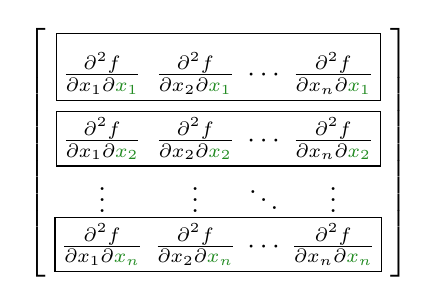
\begin{tikzpicture}[baseline=(current bounding box.center)]
		\matrix (m) [matrix of math nodes, inner sep=2pt, left delimiter={[}, right delimiter={]}] {
			|[minimum height=1cm]| \frac{\partial^2 f}{\partial x_1 \partial \textcolor{forestgreen}{x_1}} & \frac{\partial^2 f}{\partial x_2 \partial \textcolor{forestgreen}{x_1}} & \cdots & \frac{\partial^2 f}{\partial x_n \partial \textcolor{forestgreen}{x_1}} \\
			\frac{\partial^2 f}{\partial x_1 \partial \textcolor{forestgreen}{x_2}} & \frac{\partial^2 f}{\partial x_2 \partial \textcolor{forestgreen}{x_2}} & \cdots & \frac{\partial^2 f}{\partial x_n \partial \textcolor{forestgreen}{x_2}} \\
			\vdots & \vdots & \ddots & \vdots \\
			\frac{\partial^2 f}{\partial x_1 \partial \textcolor{forestgreen}{x_n}} & \frac{\partial^2 f}{\partial x_2 \partial \textcolor{forestgreen}{x_n}} & \cdots & \frac{\partial^2 f}{\partial x_n \partial \textcolor{forestgreen}{x_n}} \\
		};
		\foreach \i in {1,2,4} {
			\draw (m-\i-1.north west) rectangle (m-\i-4.south east);
		}
	\end{tikzpicture} .
	\end{aligned}
	\]
	
	\item Similarly, the second order gradient of scalar is
	\[ \begin{aligned}
	\nabla^{2} \Big( f(\boldsymbol{x}) \Big)
	& = \nabla \Big(  \nabla f \left( \boldsymbol{x} \right)^{\top} \Big)
	= \nabla \Big( D f(\boldsymbol{x}) \Big) 
	= \nabla \Big( \left[
		\begin{array}{cccc}
		\frac{\partial f}{ \color{forestgreen}{\partial x_{1}} } &
		\frac{\partial f}{ \color{forestgreen}{\partial x_{2}} } & 
		\cdots &
		\frac{\partial f}{ \color{forestgreen}{\partial x_{n}} } \end{array}\right] \Big) \\
	& = \left[\begin{array}{cccc}
		& & &  \\
		& & &  \\
		\nabla \left(\frac{\partial f}{ \color{forestgreen}{\partial x_{1}} }\right) &    
		\nabla \left(\frac{\partial f}{ \color{forestgreen}{\partial x_{2}} }\right) &    
		\cdots &    
		\nabla \left(\frac{\partial f}{ \color{forestgreen}{\partial x_{n}} }\right) \\ 
		& & & \\
		& & &  \\
	\end{array}
	\right]
	=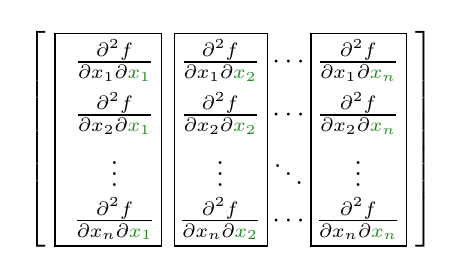
\begin{tikzpicture}[baseline=(current bounding box.center)]
		\matrix (m) [matrix of math nodes, inner sep=2pt, left delimiter={[}, right delimiter={]}] {
			|[minimum width=1.5cm]| \frac{\partial^2 f}{\partial x_1 \partial \textcolor{forestgreen}{x_1}} & \frac{\partial^2 f}{\partial x_1 \partial \textcolor{forestgreen}{x_2}} & \cdots & \frac{\partial^2 f}{\partial x_1 \partial \textcolor{forestgreen}{x_n}} \\
			\frac{\partial^2 f}{\partial x_2 \partial \textcolor{forestgreen}{x_1}} & \frac{\partial^2 f}{\partial x_2 \partial \textcolor{forestgreen}{x_2}} & \cdots & \frac{\partial^2 f}{\partial x_2 \partial \textcolor{forestgreen}{x_n}} \\
			\vdots & \vdots & \ddots & \vdots \\
			\frac{\partial^2 f}{\partial x_n \partial \textcolor{forestgreen}{x_1}} & \frac{\partial^2 f}{\partial x_n \partial \textcolor{forestgreen}{x_2}} & \cdots & \frac{\partial^2 f}{\partial x_n \partial \textcolor{forestgreen}{x_n}} \\
		};
		\foreach \i in {1,2,4} {
			\draw (m-1-\i.north west) rectangle (m-4-\i.south east);
		}
	\end{tikzpicture} .
	\end{aligned}
	\]
	

\end{itemize}


%------------------------------------------------------%
\subsection{Differentiation product rules}

\textbf{i)} Let \(f: \mathbb{R} \rightarrow \mathbb{R}\) and \(g: \mathbb{R} \rightarrow \mathbb{R}\) be two differentiable functions, \(x \in \mathbb{R}\),
\[ 
\begin{aligned}
	D \bigg (f(x) g(x) \bigg )
	& = f(x)  D g(x)
	+g(x)  D f(x),  \\
	\nabla \bigg (f(x) g(x) \bigg )
	& = f(x)  \nabla g(x)
	+g(x)  \nabla f(x). 
\end{aligned}
\]

\noindent
\textbf{ii)} Let \(f: \mathbb{R}^{n} \rightarrow \mathbb{R}\) and \(g: \mathbb{R}^{n} \rightarrow \mathbb{R}\) be two differentiable functions, \(\boldsymbol{x} \in \mathbb{R}^{n}\),
\[ 
\begin{aligned}
	D \bigg (f(\boldsymbol{x}) g(\boldsymbol{x}) \bigg )
	& = f(\boldsymbol{x}) \big [\begin{array}{ccc}
		&D g(\boldsymbol{x}) & \end{array} \big ] 
	+g(\boldsymbol{x}) \big [\begin{array}{ccc} & D f(\boldsymbol{x}) &
	\end{array} \big ], \\
	\nabla \bigg (f(\boldsymbol{x}) g(\boldsymbol{x}) \bigg )
	& = f(\boldsymbol{x}) \left [\begin{array}{c}
		\\ \nabla g(\boldsymbol{x}) \\  \\ \end{array} \right ] 
	+g(\boldsymbol{x}) \left [\begin{array}{c} \\ \nabla f(\boldsymbol{x}) \\ \\
	\end{array} \right ].
\end{aligned}
\]

\noindent
\textbf{iii)} Let \( \boldsymbol{f}: \mathbb{R}^{n} \rightarrow \mathbb{R}^{m}\) and \( \boldsymbol{g}: \mathbb{R}^{n} \rightarrow \mathbb{R}^{m}\) be two differentiable functions, \(\boldsymbol{x} \in \mathbb{R}^{n}\),
\[ 
\begin{aligned}
	D \bigg (\boldsymbol{f}(\boldsymbol{x})^{\top} \boldsymbol{g}(\boldsymbol{x}) \bigg )
	& = \left[ \begin{array}{ccc} & \boldsymbol{f}(\boldsymbol{x})^{\top} & \end{array} \right]
		\left[ \begin{array}{ccc} & & \\ & D \boldsymbol{g}(\boldsymbol{x}) & \\ & & \end{array} \right]
		+ \left[ \begin{array}{ccc} & \boldsymbol{g}(\boldsymbol{x})^{\top} & \end{array} \right]
		\left[ \begin{array}{ccc} & & \\ & 	D \boldsymbol{f}(\boldsymbol{x})  & \\ & & \end{array} \right], \\
	\nabla \bigg (\boldsymbol{f}(\boldsymbol{x})^{\top} \boldsymbol{g}(\boldsymbol{x}) \bigg )
	& = \left[ \begin{array}{ccc} & & \\ &  \nabla \boldsymbol{f}(\boldsymbol{x}) & \\ & & \end{array} \right]
		\left[\begin{array}{c}\\  \boldsymbol{g}(\boldsymbol{x}) \\  \\ \end{array} \right ] 
   		+ \left[ \begin{array}{ccc} & & \\ &  \nabla \boldsymbol{g} (\boldsymbol{x}) & \\ & & \end{array} \right]
   		\left[\begin{array}{c}\\  \boldsymbol{f}(\boldsymbol{x}) \\  \\ \end{array} \right] . \\
\end{aligned}
\]


%------------------------------------------------------%
\subsection{Differentiation rules}

\begin{itemize}
	\item If \(f=\boldsymbol{x}^{\top} \boldsymbol{Q} \boldsymbol{x}\) is a scalar, \(f^{\top}=f\).
	
	\item If \(\mathbf{Q}\) is not symmetric, we can always replace it with a symmetric matrix, 
	\[
	\left(\boldsymbol{x}^{\top} \mathbf{Q} \boldsymbol{x}\right)^{\top}=\boldsymbol{x}^{\top} \mathbf{Q}^{\top} \boldsymbol{x}=\boldsymbol{x}^{\top} \mathbf{Q} \boldsymbol{x} .
	\]
	
	Continue with manipulations,
	\[
	\boldsymbol{x}^{\top} \mathbf{Q} \boldsymbol{x}=\frac{1}{2} \boldsymbol{x}^{\top} \mathbf{Q} \boldsymbol{x}+\frac{1}{2} \boldsymbol{x}^{\top} \mathbf{Q x}=\boldsymbol{x}^{\top}\left(\frac{\mathbf{Q}+\mathbf{Q}^{\top}}{2}\right) \boldsymbol{x},
	\]
	where \(\frac{1}{2}\left(\mathbf{Q}+\mathbf{Q}^{\top}\right) = \frac{1}{2}\left(\mathbf{Q}+\mathbf{Q}^{\top}\right)^{\top}\) is a symmetric matrix.
	
	
	\item Based on the above \textbf{derivative} rule, we have

	\textbf{1.} Consider \(\mathbf{A} \in \mathbb{R}^{m \times n}\) be a given matrix and \(\boldsymbol{y} \in \mathbb{R}^{m}\) a given vector. Then,
	\begin{align*}
		D\left(\boldsymbol{y}^{\top} \mathbf{A} \boldsymbol{x}\right) &=
		\boldsymbol{y}^{\top} \mathbf{A}, \\
		D\left(\boldsymbol{x}^{\top} \mathbf{A} \boldsymbol{x}\right) &=
		\boldsymbol{x}^{\top}\left(\mathbf{A}+\mathbf{A}^{\top}\right).  \qquad
		\fbox{\parbox{0.1\textwidth}{ if \(m=n\) }}
	\end{align*}
	
	
	\textbf{2.} Consider \(\mathbf{A} \in \mathbb{R}^{m \times n}\) be a given matrix and \(\boldsymbol{y} \in \mathbb{R}^{n}\) a given vector. Then,
	\[ D\left(\boldsymbol{y}^{\top} \boldsymbol{x}\right)=\boldsymbol{y}^{\top}. \]
	
	\textbf{3.} Consider if \(\mathbf{Q}\) is a symmetric matrix, then
	\[
	D\left(\boldsymbol{x}^{\top} \mathbf{Q} \boldsymbol{x}\right)=2 \boldsymbol{x}^{\top} \mathbf{Q}.
	\]
	
	In particular,
	\[
	D\left(\boldsymbol{x}^{\top} \boldsymbol{x}\right)=2 \boldsymbol{x}^{\top}.
	\]

	\item Based on the above \textbf{gradient} rule, we have

	\textbf{1.} Consider \(\mathbf{A} \in \mathbb{R}^{m \times n}\) be a given matrix and \(\boldsymbol{y} \in \mathbb{R}^{m}\) a given vector. Then,
	\begin{align*}
		\nabla \left(\boldsymbol{y}^{\top} \mathbf{A} \boldsymbol{x}\right) &= \mathbf{A}^{\top} \boldsymbol{y}, \\
		\nabla  \left(\boldsymbol{x}^{\top} \mathbf{A} \boldsymbol{x}\right) &=
		\left(\mathbf{A}+\mathbf{A}^{\top}\right) \boldsymbol{x}.  \qquad
		\fbox{\parbox{0.1\textwidth}{ if \(m=n\) }}
	\end{align*}
	
	
	\textbf{2.} Consider \(\mathbf{A} \in \mathbb{R}^{m \times n}\) be a given matrix and \(\boldsymbol{y} \in \mathbb{R}^{n}\) a given vector. Then,
	\[ \nabla \left(\boldsymbol{y}^{\top} \boldsymbol{x}\right)=\boldsymbol{y}. \]
	
	\textbf{3.} Consider if \(\mathbf{Q}\) is a symmetric matrix, then
	\[
	\nabla \left(\boldsymbol{x}^{\top} \mathbf{Q} \boldsymbol{x}\right)=2  \mathbf{Q} \boldsymbol{x}.
	\]
	
	In particular,
	\[
	\nabla \left(\boldsymbol{x}^{\top} \boldsymbol{x}\right)=2 \boldsymbol{x}.
	\]

\end{itemize}


%------------------------------------------------------%
\subsection{Derivative details}

\begin{itemize}
	\item Let \(\boldsymbol{f}: \mathbb{R}^{n} \rightarrow \mathbb{R}^{m}\) and \(\boldsymbol{g}: \mathbb{R}^{n} \rightarrow \mathbb{R}^{m}\) be two differentiable functions, \(\boldsymbol{x} \in \mathbb{R}^{n}\),
	\[ D \bigg (\boldsymbol{f}(\boldsymbol{x})^{\top} \boldsymbol{g}(\boldsymbol{x}) \bigg )
	=\boldsymbol{f}(\boldsymbol{x})^{\top} D \boldsymbol{g}(\boldsymbol{x})+\boldsymbol{g}(\boldsymbol{x})^{\top} D \boldsymbol{f}(\boldsymbol{x}). \]
	
	We can write it into compact matrix form as,
	\[
	\begin{aligned}
		D\left( \sideset{^{1 \backslash m}}{}{ 
			\left. \boldsymbol{\Big[}
			\begin{array}{ccc} & \boldsymbol{f}(\boldsymbol{x})^{\top} & \end{array} 
			\boldsymbol{\Big]}
			\right.
			}
		\sideset{^{m \backslash 1}}{}{ 
			\left[ \begin{array}{c} \\ \boldsymbol{g}(\boldsymbol{x}) \\ \\ \end{array} \right]
		}
		\right)
		& = \hspace{0.6cm}
		\left. \sideset{^{1 \backslash m}}{}{
			\left[ \begin{array}{ccc} & \boldsymbol{f}(\boldsymbol{x})^{\top} & \end{array} \right]
		}
		\sideset{^{m \backslash n}}{}{
			\left[ \begin{array}{c} \\ D \boldsymbol{g}(\boldsymbol{x}) \\ \\ \end{array} \right]
		}
		\right. \\
		&  \hspace{0.7cm} +
		\left. \sideset{^{1 \backslash m}}{}{
			\left[ \begin{array}{ccc} & \boldsymbol{g}(\boldsymbol{x})^{\top} & \end{array} \right]
		}
		\sideset{^{m \backslash n}}{}{
			\left[ \begin{array}{c} \\ D\boldsymbol{f}(\boldsymbol{x}) \\ \\ \end{array} \right].
		}
		\right.
	\end{aligned}
	\]

	\textbf{Short proof},
	
	\(\boldsymbol{f}: \mathbb{R}^{n} \rightarrow \mathbb{R}^{\color{forestgreen}{m}}\) and \(\boldsymbol{g}: \mathbb{R}^{n} \rightarrow \mathbb{R}^{\color{forestgreen}{m}}\), \(\boldsymbol{x} \in \mathbb{R}^{n}\), write the derivative as 
		\[\begin{aligned}
		D \Big(\boldsymbol{f}(\boldsymbol{x})^{\top} \boldsymbol{g}(\boldsymbol{x})\Big)
		&=D \left(
		\boldsymbol{\Big[} \begin{array}{ccc}
			f_{1}(\boldsymbol{x}) & \cdots & f_{\color{forestgreen}{m}}(\boldsymbol{x})
		\end{array}
		\boldsymbol{\Big]}
		\left[ \begin{array}{c}
			g_{1}(\boldsymbol{x}) \\ \vdots \\ g_{\color{forestgreen}{m}}(\boldsymbol{x})
		\end{array}
		\right]
		\right)
		\\
		& \\
		&=D \left(
		\boldsymbol{\Big[} \begin{array}{ccc}
			f_{1} \left(x_{1}, x_{2}, \ldots, x_{n}\right) 
			& \cdots 
			& f_{\color{forestgreen}{m}}\left(x_{1}, x_{2}, \ldots, x_{n}\right)
		\end{array}
		\boldsymbol{\Big]}
		\left[ \begin{array}{cc}
			g_{1}\left(x_{1}, x_{2}, \ldots, x_{n}\right) \\
			\vdots \\
			g_{\color{forestgreen}{m}}\left(x_{1}, x_{2}, \ldots, x_{n}\right)
		\end{array}
		\right] \right)\\
		& \\
		& = D \Big(
		f_{1}(\boldsymbol{x})g_{1}(\boldsymbol{x}) + \cdots + 
		f_{\color{forestgreen}{m}}(\boldsymbol{x})g_{\color{forestgreen}{m}}(\boldsymbol{x})
		\Big) \\
		& \\
		& =  f_{1}(\boldsymbol{x})D g_{1}(\boldsymbol{x}) + \cdots +
		f_{\color{forestgreen}{m}}(\boldsymbol{x})D g_{\color{forestgreen}{m}}(\boldsymbol{x}) \\
		& \hspace{7 cm}
		+ g_{1}(\boldsymbol{x})D f_{1}(\boldsymbol{x}) + \cdots +
		g_{\color{forestgreen}{m}}(\boldsymbol{x})D f_{\color{forestgreen}{m}}(\boldsymbol{x}) \\
		& \\
		& = \left.
		\boldsymbol{\Big[} \begin{array}{ccc}
			f_{1}(\boldsymbol{x}) & \cdots & f_{\color{forestgreen}{m}}(\boldsymbol{x})
		\end{array}
		\boldsymbol{\Big]}
		\left[ \begin{array}{c}
			D g_{1}(\boldsymbol{x}) \\ \vdots \\ D g_{\color{forestgreen}{m}}(\boldsymbol{x})
		\end{array}
		\right]
		\right. +
		\left.
		\boldsymbol{\Big[} \begin{array}{ccc}
			g_{1}(\boldsymbol{x}) & \cdots & g_{\color{forestgreen}{m}}(\boldsymbol{x})
		\end{array}
		\boldsymbol{\Big]}
		\left[ \begin{array}{c}
			D f_{1}(\boldsymbol{x}) \\ \vdots \\ D f_{\color{forestgreen}{m}}(\boldsymbol{x})
		\end{array}
		\right]
		\right. \\
		\end{aligned}\]
	
		\[\begin{aligned}
		{\color{white}D \Big(\boldsymbol{f}(\boldsymbol{x})^{\top} \boldsymbol{g}(\boldsymbol{x})\Big)}
		& = 
		\left. \sideset{^{1 \backslash m}}{}{
			\left[
			\begin{array}{ccc} & \boldsymbol{f}(\boldsymbol{x})^{\top} & \end{array}
			\right]
			}
		\sideset{^{m \backslash n}}{}{
			\left[ \begin{array}{c} \\ D \boldsymbol{g}(\boldsymbol{x}) \\ \\ \end{array} \right]
			}
		\right. +
		\left. \sideset{^{1 \backslash m}}{}{
			\left[
			\begin{array}{ccc} & \boldsymbol{g}(\boldsymbol{x})^{\top} & \end{array}
			\right]
			}
		\sideset{^{m \backslash n}}{}{
			\left[ \begin{array}{c} \\ D\boldsymbol{f}(\boldsymbol{x}) \\ \\ \end{array} \right]
			}
		\right. . \\
	\end{aligned}\]
	
	\vspace{5cm}

	\item Let \(\mathbf{A} \in \mathbb{R}^{m \times n}\) be a given matrix and \(\boldsymbol{y} \in \mathbb{R}^{m}\) a given vector. Then,
	\begin{align*}
		D\left(\boldsymbol{y}^{\top} \mathbf{A} \boldsymbol{x}\right) &=
		\boldsymbol{y}^{\top} \mathbf{A}, \\
		D\left(\boldsymbol{x}^{\top} \mathbf{A} \boldsymbol{x}\right) &=
		\boldsymbol{x}^{\top}\left(\mathbf{A}+\mathbf{A}^{\top}\right).  \qquad
		\fbox{\parbox{0.1\textwidth}{ if \(m=n\) }}
	\end{align*}
	
	\textbf{Short proof},
	\[\begin{aligned}    
		D\left(\boldsymbol{y}^{\top} \mathbf{A} \boldsymbol{x}\right) 
		&=D \bigg ( \boldsymbol{y}^{\top}( {\color{forestgreen}{\mathbf{A} \boldsymbol{x}}} ) \bigg )
		=D \bigg ( \boldsymbol{f}(\boldsymbol{y})^{\top} \Big( {\color{forestgreen}{\boldsymbol{g}(\boldsymbol{x})}} \Big) \bigg ) \\    
		&=\boldsymbol{f}(\boldsymbol{y})^{\top} D \boldsymbol{g} (\boldsymbol{x})
		+\boldsymbol{g}(\boldsymbol{x})^{\top} D \boldsymbol{f}(\boldsymbol{y}) \\    
		&=\boldsymbol{y}^{\top} D(\mathbf{A} \boldsymbol{x})+(\mathbf{A} \boldsymbol{x})^{\top}[\mathbf{0}] \\
		&=\boldsymbol{y}^{\top} \mathbf{A}.
	\end{aligned}\]
	If \(\mathbf{A} \in \mathbb{R}^{n \times n}\),
	\[ \begin{aligned}    
		D\left(\boldsymbol{x}^{\top} \mathbf{A} \boldsymbol{x}\right)    
		&=D \bigg( \boldsymbol{x}^{\top}( {\color{forestgreen}{\mathbf{A} \boldsymbol{x}}} ) \bigg)
		=D\bigg(\boldsymbol{f}(\boldsymbol{x})^{\top} \Big( {\color{forestgreen}{\boldsymbol{g}(\boldsymbol{x})}} \Big ) \bigg) \\     
		&=\boldsymbol{f}(\boldsymbol{x})^{\top} D \boldsymbol{g} (\boldsymbol{x})+\boldsymbol{g}(\boldsymbol{x})^{\top} D \boldsymbol{f}(\boldsymbol{x}) \\    
		&=\boldsymbol{x}^{\top} D(\mathbf{A} \boldsymbol{x})+(\mathbf{A} \boldsymbol{x})^{\top} D(\mathbf{I}_{n} \boldsymbol{x}) \\    
		&=\boldsymbol{x}^{\top} \mathbf{A}+\boldsymbol{x}^{\top} \mathbf{A}^{\top} \mathbf{I}  \\
		&=\boldsymbol{x}^{\top} \left(\mathbf{A}+\mathbf{A}^{\top}\right).
	\end{aligned} \]

	\item It follows that if \(\mathbf{Q}\) is a symmetric matrix, then
	\[ \begin{aligned}
		D\left(\boldsymbol{x}^{\top} \mathbf{Q} \boldsymbol{x}\right) &=2 \boldsymbol{x}^{\top} \mathbf{Q}, \\
		D\left(\boldsymbol{x}^{\top} \boldsymbol{x}\right) &=2 \boldsymbol{x}^{\top}.
	\end{aligned}
	\]
	
	\textbf{Short proof},
	\[ \begin{aligned}    
		D\left(\boldsymbol{x}^{\top} \mathbf{Q} \boldsymbol{x}\right)    
		&=D \bigg( \boldsymbol{x}^{\top}( {\color{forestgreen}{\mathbf{Q} \boldsymbol{x}}} ) \bigg) \\
		&=\boldsymbol{x}^{\top} \left(\mathbf{Q}+\mathbf{Q}^{\top}\right) \\
		&=2 \boldsymbol{x}^{\top} \mathbf{Q},
	\end{aligned} \]
	\[ \begin{aligned}    
		D\left(\boldsymbol{x}^{\top}  \boldsymbol{x}\right)
		&=D\left(\boldsymbol{x}^{\top} \mathbf{I} \boldsymbol{x}\right) 
		=D \bigg( \boldsymbol{x}^{\top}( {\color{forestgreen}{\mathbf{I} \boldsymbol{x}}} ) \bigg) \\
		&=\boldsymbol{x}^{\top} \left(\mathbf{I}+\mathbf{I}^{\top}\right) \\
		&=2 \boldsymbol{x}^{\top}.
	\end{aligned} \]

	\item Derivative of scalar by scalar,
	\[\begin{aligned}
		\frac{\mathrm{d}}{\mathrm{d} \alpha}\left((\alpha \boldsymbol{x})^{\top} \mathbf{Q}(\alpha \boldsymbol{x})\right) 
		&=(\alpha \boldsymbol{x})^{\top} \frac{\mathrm{d}}{\mathrm{d} \alpha}(\mathbf{Q}(\alpha \boldsymbol{x}))
		+(\mathbf{Q}(\alpha \boldsymbol{x}))^{\top} \frac{\mathrm{d}}{\mathrm{d} \alpha}(\mathbf{I}(\alpha \boldsymbol{x})) \\
		& =(\alpha \boldsymbol{x})^{\top} \mathbf{Q} \boldsymbol{x}+(\alpha \boldsymbol{x})^{\top} \mathbf{Q}^{\top} \boldsymbol{x} \\
		& = 2 (\alpha \boldsymbol{x})^{\top} \mathbf{Q} \boldsymbol{x} \\
		& = 2 \alpha \boldsymbol{x}^{\top} \mathbf{Q} \boldsymbol{x} \\
	\end{aligned}
	\]
\end{itemize}


\newpage
%------------------------------------------------------%
\subsection{Gradient details}
\begin{itemize}
	\item Consider \(\boldsymbol{g}: \mathbb{R}^{n} \rightarrow \mathbb{R}^m \),  here \( \boldsymbol{x} \in  \mathbb{R}^n \) is a vector. Since \(g_{i}(\boldsymbol{x})\) is a scalar, \(\boldsymbol{g}=\left[g_1, \ldots, g_m\right]^{\top} \), \(\boldsymbol{g}(\boldsymbol{x})\) is a column vector. 
	\[
	\begin{aligned}
		\boldsymbol{g} \left( \boldsymbol{x} \right)=
		\left[
		\begin{array}{c}
			g_{1}( \boldsymbol{x} ) \\
			g_{2}( \boldsymbol{x} ) \\
			\vdots \\
			g_{m}( \boldsymbol{x} )
		\end{array}
		\right], 
		\nabla_{\boldsymbol{x}} \boldsymbol{g}\left( \boldsymbol{x} \right) & =\left[
		\begin{array}{ccc}
			\vdots & \vdots & \vdots \\
			{ \color{blue}\nabla_{\boldsymbol{x}} } g_{1} &
			\cdots &
			{ \color{blue}\nabla_{\boldsymbol{x}} } g_{m} \\
			\vdots & \vdots & \vdots \\
		\end{array}
		\right]
		= 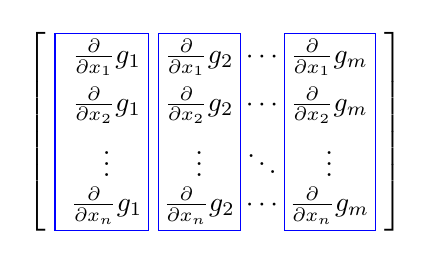
\begin{tikzpicture}[baseline=(current bounding box.center)]
			\tikzset{
				mynode/.style={minimum height=1cm}
			}
			\matrix [matrix of math nodes, inner sep=2pt, left delimiter={[},right delimiter={]}] (m) {
				|[minimum width=1.3cm]| \frac{\partial}{\partial x_1} g_1 & \frac{\partial}{\partial x_1} g_2 & \cdots & \frac{\partial}{\partial x_1} g_m \\
				\frac{\partial}{\partial x_2} g_1 & \frac{\partial}{\partial x_2} g_2 & \cdots & \frac{\partial}{\partial x_2} g_m \\
				\vdots & \vdots & \ddots & \vdots \\
				\frac{\partial}{\partial x_n} g_1 & \frac{\partial}{\partial x_n} g_2 & \cdots & \frac{\partial}{\partial x_n} g_m \\
			};
			\draw[blue] (m-1-1.north west) rectangle (m-4-1.south east);
			\draw[blue] (m-1-2.north west) rectangle (m-4-2.south east);
			\draw[blue] (m-1-4.north west) rectangle (m-4-4.south east);
		\end{tikzpicture}.
	\end{aligned}
	\]
	
	\item Not standard derivations in this course, just offer some intuitions on how to obtained the gradients on production rules.
	
	\item Let \(\boldsymbol{f}: \mathbb{R}^{n} \rightarrow \mathbb{R}^{m}\) and \(\boldsymbol{g}: \mathbb{R}^{n} \rightarrow \mathbb{R}^{m}\) be two differentiable functions, \(\boldsymbol{x} \in \mathbb{R}^{n}\),
	\[ 	\nabla \bigg (\boldsymbol{f}(\boldsymbol{x})^{\top} \boldsymbol{g}(\boldsymbol{x}) \bigg )
	 = \nabla \boldsymbol{f}(\boldsymbol{x}) \left[\begin{array}{c}\\  \boldsymbol{g}(\boldsymbol{x}) \\  \\ \end{array} \right] 
	+ \nabla\boldsymbol{g} (\boldsymbol{x}) \left[\begin{array}{c}\\  f(\boldsymbol{x}) \\  \\ \end{array} \right]. \]
	
	Proof. 
	\(\boldsymbol{f}: \mathbb{R}^{n} \rightarrow \mathbb{R}^{\color{forestgreen}{m}}\) and \(\boldsymbol{g}: \mathbb{R}^{n} \rightarrow \mathbb{R}^{\color{forestgreen}{m}}\), \(\boldsymbol{x} \in \mathbb{R}^{n}\), write the derivative as 
	\[\begin{aligned}
		\nabla \Big(\boldsymbol{f}(\boldsymbol{x})^{\top} \boldsymbol{g}(\boldsymbol{x})\Big)
		&=\nabla \left(
		\boldsymbol{\Big[} \begin{array}{ccc}
			f_{1}(\boldsymbol{x}) & \cdots & f_{\color{forestgreen}{m}}(\boldsymbol{x})
		\end{array}
		\boldsymbol{\Big]}
		\left[ \begin{array}{c}
			g_{1}(\boldsymbol{x}) \\ \vdots \\ g_{\color{forestgreen}{m}}(\boldsymbol{x})
		\end{array}
		\right]
		\right)
		\\
		&=\nabla \left(
		\boldsymbol{\Big[} \begin{array}{ccc}
			f_{1} \left(x_{1}, x_{2}, \ldots, x_{n}\right) 
			& \cdots 
			& f_{\color{forestgreen}{m}}\left(x_{1}, x_{2}, \ldots, x_{n}\right)
		\end{array}
		\boldsymbol{\Big]}
		\left[ \begin{array}{cc}
			g_{1}\left(x_{1}, x_{2}, \ldots, x_{n}\right) \\
			\vdots \\
			g_{\color{forestgreen}{m}}\left(x_{1}, x_{2}, \ldots, x_{n}\right)
		\end{array}
		\right] \right)\\
		& \\
		& = \nabla \Big(
		f_{1}(\boldsymbol{x})g_{1}(\boldsymbol{x}) + \cdots + 
		f_{\color{forestgreen}{m}}(\boldsymbol{x})g_{\color{forestgreen}{m}}(\boldsymbol{x})
		\Big) \\
		& \\
		& =  f_{1}(\boldsymbol{x})\nabla g_{1}(\boldsymbol{x}) + \cdots +
		f_{\color{forestgreen}{m}}(\boldsymbol{x})\nabla g_{\color{forestgreen}{m}}(\boldsymbol{x}) \\
		& \hspace{7.3cm}
		+ g_{1}(\boldsymbol{x})\nabla f_{1}(\boldsymbol{x}) + \cdots +
		g_{\color{forestgreen}{m}}(\boldsymbol{x})\nabla f_{\color{forestgreen}{m}}(\boldsymbol{x}) \\
		& \\
		& = \left.
			\boldsymbol{\Big[} \begin{array}{ccc}
				\nabla g_{1}(\boldsymbol{x}) & \cdots & \nabla g_{\color{forestgreen}{m}}(\boldsymbol{x})
			\end{array}
			\boldsymbol{\Big]}
			\left[ \begin{array}{c}
				f_{1}(\boldsymbol{x}) \\ \vdots \\ f_{\color{forestgreen}{m}}(\boldsymbol{x})
			\end{array}
			\right]
			\right. +
			\left.
			\boldsymbol{\Big[} \begin{array}{ccc}
				\nabla f_{1}(\boldsymbol{x}) & \cdots & \nabla f_{\color{forestgreen}{m}}(\boldsymbol{x})
			\end{array}
			\boldsymbol{\Big]}
			\left[ \begin{array}{c}
				g_{1}(\boldsymbol{x}) \\ \vdots \\ g_{\color{forestgreen}{m}}(\boldsymbol{x})
			\end{array}
			\right]
			\right. \\
		& \\
		& = \underbrace{\boldsymbol{f}(\boldsymbol{x})^{\top}}_{1 \times m} \underbrace{D \boldsymbol{g}(\boldsymbol{x})}_{m \times n}+\underbrace{\boldsymbol{g}(\boldsymbol{x})^{\top}}_{1 \times m} \underbrace{D \boldsymbol{f}(\boldsymbol{x})}_{m \times n} \\
		& \\
		& =  \left.
			\boldsymbol{\Big[} \begin{array}{ccc}
				\nabla f_{1}(\boldsymbol{x}) & \cdots & \nabla f_{\color{forestgreen}{m}}(\boldsymbol{x})
			\end{array}
			\boldsymbol{\Big]}
			\left[ \begin{array}{c}
				g_{1}(\boldsymbol{x}) \\ \vdots \\ g_{\color{forestgreen}{m}}(\boldsymbol{x})
			\end{array}
			\right]
			\right. + 
			\left.
			\boldsymbol{\Big[} \begin{array}{ccc}
				\nabla g_{1}(\boldsymbol{x}) & \cdots & \nabla g_{\color{forestgreen}{m}}(\boldsymbol{x})
			\end{array}
			\boldsymbol{\Big]}
			\left[ \begin{array}{c}
				f_{1}(\boldsymbol{x}) \\ \vdots \\ f_{\color{forestgreen}{m}}(\boldsymbol{x})
			\end{array}
			\right]
			\right.\\
	\end{aligned}\]

	\[\begin{aligned}
	{\color{white} \nabla \Big(\boldsymbol{f}(\boldsymbol{x})^{\top} \boldsymbol{g}(\boldsymbol{x})\Big)}
	& = \left. 
		\sideset{^{n \backslash m}}{}{
			\left[
			\begin{array}{ccc}  & &\\ &  \nabla \boldsymbol{f}(\boldsymbol{x}) & \\  & & \\  \end{array}
			\right]
		}
		\sideset{^{m \backslash 1}}{}{
			\left[ \begin{array}{c} \\  \boldsymbol{g}(\boldsymbol{x}) \\ \\ \end{array} \right]
		}
		\right. +
		\left. 
		\sideset{^{n \backslash m}}{}{
			\left[ \begin{array}{ccc} & & \\ & \nabla \boldsymbol{g}(\boldsymbol{x}) & \\ & & \end{array} \right]
		}
		\sideset{^{m \backslash 1}}{}{
			\left[ \begin{array}{c} \\ \boldsymbol{f}(\boldsymbol{x}) \\ \\ \end{array} \right]
		}
		\right. \\
	\end{aligned}\]

\end{itemize}


\newpage
\begin{itemize}
	\item For example, 	if \(\mathbf{A} \in \mathbb{R}^{n \times n}\),
	
	\[ \begin{aligned}    
		\nabla \left(\boldsymbol{x}^{\top} \mathbf{A} \boldsymbol{x}\right)    
		&=\nabla \bigg( \boldsymbol{x}^{\top}( {\color{black}{\mathbf{A} \boldsymbol{x}}} ) \bigg) \\ 
		&=\nabla \left(
		\boldsymbol{\Big[} \begin{array}{ccc}
			x_{1} & \cdots & x_{n}
		\end{array}
		\boldsymbol{\Big]}
		\left[ \begin{array}{c}
			\boldsymbol{a}_{1}^{\top}\boldsymbol{x} \\ \vdots \\ \boldsymbol{a}_{n}^{\top}\boldsymbol{x}
		\end{array}
		\right]
		\right)
		\\
		& \\
		&=\nabla \bigg( x_{1}\boldsymbol{a}_{1}^{\top}\boldsymbol{x} + \cdots + x_{n}\boldsymbol{a}_{n}^{\top}\boldsymbol{x} \bigg) \\
		& \\
		&= {\color{forestgreen} x_{1} \nabla (\boldsymbol{a}_{1}^{\top}\boldsymbol{x}) + \cdots + x_{n} \nabla (\boldsymbol{a}_{n}^{\top}\boldsymbol{x})} \\
		& \quad + \boldsymbol{a}_{1}^{\top}\boldsymbol{x} \nabla \bigg(1x_{1}+0x_{2}+ \cdots+ 0x_{n}\bigg) + \cdots +  \boldsymbol{a}_{n}^{\top}\boldsymbol{x} \nabla \bigg( 0x_{1}+0x_{2}+ \cdots+ 1x_{n} \bigg)\\
		& \\
		&= \boldsymbol{a}_{1}^{\top}\boldsymbol{x} \left[ \begin{array}{c} 1 \\ 0 \\ \vdots \\ 0 \end{array}\right] + \cdots + \boldsymbol{a}_{n}^{\top}\boldsymbol{x} \left[ \begin{array}{c} 0 \\ 0 \\ \vdots \\ 1 \end{array}\right]
		+ {\color{forestgreen} \boldsymbol{a}_{1} x_{1} + \cdots + \boldsymbol{a}_{n} x_{n}}
		\\
		& \\
		& = \left[ \begin{array}{cccc} 
				1  & 0 & \cdots & 0 \\
				0 & 1  & \cdots & 0 \\
				\vdots  & \vdots & \ddots & \vdots   \\
				0 & 0 & \cdots & 1 
				 \end{array}\right]
			 \left[ \begin{array}{c} 
			 	\boldsymbol{a}_{1}^{\top}\boldsymbol{x} \\
			 	\boldsymbol{a}_{2}^{\top}\boldsymbol{x} \\
			 	\vdots     \\
			 	\boldsymbol{a}_{n}^{\top}\boldsymbol{x}
			 \end{array}\right] 
		  + \boldsymbol{\Big[} \begin{array}{cccc}
			  	\boldsymbol{a}_{1} & \boldsymbol{a}_{2} & \cdots & \boldsymbol{a}_{n}
			  \end{array}
			  \boldsymbol{\Big]}
			  \left[ \begin{array}{c} x_{1} \\ x_{2} \\ \vdots \\ x_{n} \end{array}\right]
		\\
		& \\
		&= \left[ \begin{array}{ccc} && \\  &\mathbf{I}& \\ &&\\ \end{array} \right]
			\left[ \begin{array}{c} \\  \mathbf{A}\boldsymbol{x} \\ \\ \end{array} \right]
		  + \left[ \begin{array}{ccc} && \\  &\mathbf{A}^{\top}& \\ &&\\ \end{array} \right]
		  	\left[ \begin{array}{c} \\ \boldsymbol{x} \\ \\ \end{array} \right] 
		  	= \left( \mathbf{A} + \mathbf{A}^{\top} \right) \boldsymbol{x}
		\\
		& \\
		& = \left[
			\begin{array}{ccc}  & &\\ &  \nabla \boldsymbol{f}(\boldsymbol{x}) & \\  & & \\  \end{array}
			\right]
		{\left[ \begin{array}{c} \\  \boldsymbol{g}(\boldsymbol{x}) \\ \\ \end{array} \right]} +
			\left[
			\begin{array}{ccc} & &\\ & \nabla \boldsymbol{g}(\boldsymbol{x}) & \\ & & \end{array}
			\right]
		{\left[ \begin{array}{c} \\ \boldsymbol{f}(\boldsymbol{x}) \\ \\ \end{array} \right]} \\
		& \\
		& = \nabla \Big(\boldsymbol{f}(\boldsymbol{x})^{\top} \boldsymbol{g}(\boldsymbol{x})\Big),
	\end{aligned} \]
	
	where \(\boldsymbol{f}(\boldsymbol{x})=\boldsymbol{x}\), \(\boldsymbol{g}(\boldsymbol{x})=\mathbf{A}\boldsymbol{x} \).
\end{itemize}

\newpage
\begin{itemize}
	\item Hand writing derivation: given
	\(\underline{y} \in \mathbb{R}^{m}, \underline{A} \in \mathbb{R}^{m \times n}, \underline{x} \in \mathbb{R}^{n}\), write the derivative as
	
	\[ 
	\begin{aligned} D_{\boldsymbol{x}}
		\left(  \boldsymbol{y}^{\top} \mathbf{A} \boldsymbol{x}
		\right) 
		&= D_{ \underline{x} } \left(  \underline{y}^{\top} \underline{A} \hspace{0.5em} \underline{x}  \right)\\
		& \\
		&=D \left( 
			\sideset{^{1 \backslash m}}{}{
				\Big[ \begin{array}{ccc} & \underline{y}^{\top} & \end{array}\Big]
			} 
			\sideset{^{m \backslash n}}{}{
				\left[ \begin{array}{ccc} & & \\ & \underline{A} & \\ & &\end{array} \right]
			}
			\sideset{^{n \backslash 1}}{}{
				\left[ \begin{array}{c}  \\  \underline{x}  \\ \\ \end{array} \right]
			}
		\right)\\
		& \\
		&=   \left. 
			\sideset{^{1 \backslash m}}{}{
				\Big[ \begin{array}{ccc} & \underline{y}^{\top} & \end{array}\Big]
			}
			\right. D \left( 
			\sideset{^{m \backslash n}}{}{
				\left[ \begin{array}{ccc} & & \\ & \underline{A} & \\ & &\end{array} \right]
			}
			\sideset{^{n \backslash 1}}{}{
				\left[ \begin{array}{c}  \\  \underline{x}  \\ \\ \end{array} \right]
			}
		\right) \\
		& \quad + \left( 
			\sideset{^{m \backslash n}}{}{
				\left[ \begin{array}{ccc} & & \\ & \underline{A} & \\ & &\end{array} \right]
			}
			\sideset{^{n \backslash 1}}{}{
				\left[ \begin{array}{c}  \\  \underline{x}  \\ \\ \end{array} \right]
			}
			\right)^{\top} 
			\left. 
			\sideset{^{m \backslash n}}{}{
				\left[ \begin{array}{ccc} & & \\ & D \underline{y} & \\ & &\end{array} \right]
			}
		\right.
		\\
		&=   
			\sideset{^{1 \backslash m}}{}{
				\Big[ \begin{array}{ccc} & \underline{y}^{\top} & \end{array}\Big]
			} 
			\sideset{^{m \backslash n}}{}{
				\left[ \begin{array}{ccc} & & \\ & \underline{A} & \\ & &\end{array} \right]
			}
			+ \sideset{^{1 \backslash n}}{}{
				\Big[ \begin{array}{ccc} & \underline{x}^{\top} & \end{array}\Big]
			} 
			\sideset{^{n \backslash m}}{}{
				\left[ \begin{array}{ccc} & & \\ & \underline{A}^{\top} & \\ & &\end{array} \right]
			}
			\sideset{^{m \backslash n}}{}{
				\left[ \begin{array}{ccc} & & \\  & \underline{0} &  \\ & & \end{array} \right]
			} \\
		&=  
			\sideset{^{1 \backslash m}}{}{
				\Big[ \begin{array}{ccc} & \underline{y}^{\top} & \end{array}\Big]
			} 
			\sideset{^{m \backslash n}}{}{
				\left[ \begin{array}{ccc} & & \\ & \underline{A} & \\ & &\end{array} \right]
			} \\
		&= \boldsymbol{y}^{\top} \mathbf{A}.
	\end{aligned} \\
	\]
\end{itemize}

%\newpage
%\begin{itemize}
%	\item Hand writing derivation: given
%	\(\underline{y} \in \mathbb{R}^{m}, \underline{A} \in \mathbb{R}^{m \times n}, \underline{x} \in \mathbb{R}^{n}\)
%
%	\[ \hspace{-1cm}
%	\begin{aligned} D_{\boldsymbol{x}}
%		\left(  \boldsymbol{y}^{\top} \mathbf{A} \boldsymbol{x}
%		\right) 
%		&= D_{ \underline{x} } \left(  \underline{y}^{\top} \underline{A} \hspace{0.5em} \underline{x}  \right)\\
%		&= D \left( 
%			\begin{matrix}
%				1 \backslash m &  \\
%				& { \begin{bmatrix} & & \underline{y}^{\top} & & \\ \end{bmatrix} } \\
%			\end{matrix}
%			\begin{matrix}
%				m \backslash n &  \\
%				& { \begin{bmatrix} & & \\ & \underline{A}  & \\ & & \end{bmatrix} } \\
%			\end{matrix}
%			\begin{matrix}
%				n \backslash 1 &  \\
%				& { \begin{bmatrix}  \\  \underline{x}  \\  \\  \end{bmatrix} } \\
%			\end{matrix}
%			\right)\\
%		&=\begin{matrix}
%				1 \backslash m &  \\
%				& { \begin{bmatrix} & & \underline{y}^{\top} & & \\ \end{bmatrix} } \\
%			\end{matrix}
%			D \left( \begin{matrix}
%				m \backslash n &  \\
%				& { \begin{bmatrix} & & \\ & \underline{A}  & \\ & & \end{bmatrix} } \\
%			\end{matrix}
%			\begin{matrix}
%				n \backslash 1 &  \\
%				& { \begin{bmatrix}  \\  \underline{x}  \\  \\  \end{bmatrix} } \\
%			\end{matrix}
%			\right)\\
%		& \quad + {\left( \begin{matrix}
%				m \backslash n &  \\
%				& { \begin{bmatrix} & & \\ & \underline{A}  & \\ & & \end{bmatrix} } \\
%			\end{matrix}
%			\begin{matrix}
%				n \backslash 1 &  \\
%				& { \begin{bmatrix}  \\  \underline{x}  \\  \\  \end{bmatrix} } \\
%			\end{matrix}
%			\right)}^{\top}
%			\begin{matrix}
%				m \backslash n &  \\
%				& { \begin{bmatrix} & & \\ & D \underline{y} & \\ & & \\ \end{bmatrix} } \\
%			\end{matrix}\\
%		&= \begin{matrix}
%				1 \backslash m &  \\
%				& { \begin{bmatrix} & & \underline{y}^{\top} & & \end{bmatrix} } \\
%			\end{matrix}
%			\begin{matrix}
%				m \backslash n &  \\
%				& { \begin{bmatrix} & & \\ & \underline{A}  & \\ & & \end{bmatrix} } \\
%			\end{matrix} +
%			\begin{matrix}
%				1 \backslash n &  \\
%				& { \begin{bmatrix} & & \underline{x}^{\top} & & \end{bmatrix} } \\
%			\end{matrix}
%			\begin{matrix}
%				n \backslash m &  \\
%				& { \begin{bmatrix} & & \\ & \underline{A}^{\top}  & \\ & & \end{bmatrix} } \\
%			\end{matrix}
%			\begin{matrix}
%				m \backslash n &  \\
%				& { \begin{bmatrix} & & \\ & \underline{0} & \\ & & \\ \end{bmatrix} } \\
%			\end{matrix}\\
%		&= \begin{matrix}
%				1 \backslash m &  \\
%				& { \begin{bmatrix} & & \underline{y}^{\top} & & \end{bmatrix} } \\
%			\end{matrix}
%			\begin{matrix}
%				m \backslash n &  \\
%				& { \begin{bmatrix} & & \\ & \underline{A}  & \\ & & \end{bmatrix} } \\
%			\end{matrix} \\
%		&= \boldsymbol{y}^{\top} \mathbf{A}.
%	\end{aligned}
%	\]
%\end{itemize}


\bigskip

\noindent
[Ref]: Edwin K.P. Chong, Stanislaw H. Żak, ``PART I MATHEMATICAL REVIEW" in ``An introduction to optimization", 4th Edition, John Wiley and Sons, Inc. 2013.



\end{document}
